%%%%%%%%%%%%%%%%%%%%%%%%%%%%%%%%%%%%%%%%%%%%%%%%%%%%%%%%%%%%%%%%%%%%%%%%%
\section{Introduction}  %%%%%%%%%%%%%%%%%%%%%%%%%%%%%%%%%%%%%%%%%%%%%%%%%
\label{cr:sec:intro}

Consider the problem of estimating click probabilities for links between pages of a website, given a hyperlink graph and aggregate statistics on the number of times each page has been visited.
Naively, one might expect that the probability of clicking on a particular link should be roughly proportional to the traffic of the link's target.
%At first, one might expect that links pointing to high-traffic web pages must be more likely to be clicked.
However, this neglects important structural effects:
a page's traffic is influenced by
\begin{enuminline}
\item the number of incoming links,
\item the traffic at the pages that link to it, and
\item the traffic absorbed by competing links.
\end{enuminline}
In order to successfully infer click probabilities, it is therefore necessary to disentangle the \emph{preference} for a page (i.e., the intrinsic propensity of a user to click on a link pointing to it) from the page's \emph{visibility} (the exposure it gets from pages linking to it).
Building upon recent work by \citet{kumar2015inverting}, we present a statistical framework that tackles a general formulation of the problem:
given a network (representing possible transitions between nodes) and the marginal traffic at each node, recover the transition probabilities.
This problem is relevant to a number of scenarios (in social, information or transportation networks) where transition data is not available due to, e.g., privacy concerns or monitoring costs.

%Our starting point is a choice model, i.e., a model that explains and predicts outcomes of comparisons between two or more alternatives from a universe of $n$ items.
%In this context, a prominent paradigm (which dates back to \citet{thurstone1927method} and \citet{zermelo1928berechnung} almost a century ago) postulates that each item can be characterized by a latent \emph{strength} parameter, and that the (stochastic) comparison outcomes tend to favor items with greater strengths.
%The parameters can be learned from observed choices and used for predicting future comparisons.
%Models based on this paradigm have been successfully applied to problems ranging from ranking chess players based on game outcomes \citep{zermelo1928berechnung, elo1978rating} to understanding consumer behavior based on discrete choices \citep{mcfadden1973conditional}, and to discriminating among multiple classes based on the output of pairwise classifiers \citep{hastie1998classification}.
%Here, we assume that the comparisons are generated from a specific stochastic process on a network, reminiscent of the random-surfer model introduced by \citet{brin1998anatomy}.
%In our setting, every node in the network represents an item, and comparisons take place over the $n$ sets of alternatives induced by the neighborhoods of each node.
We begin by postulating the following model of traffic.
Users navigate from node to node along the edges of the network by making a choice between adjacent nodes at each step, reminiscent of the random-surfer model introduced by \citet{brin1998anatomy}.
Choices are assumed to be independent and generated according to Luce's model \citep{luce1959individual}: each node in the network is chararacterized by a latent \emph{strength} parameter, and (stochastic) choice outcomes tend to favor nodes with greater strengths.
In this model, estimating the transition probabilities amounts to estimating the strength parameters.
Unlike the setting in which choice models are traditionally studied \citep{train2009discrete, maystre2015fast, vojnovic2016parameter}, we do not observe distinct choices among well-identified sets of alternatives.
Instead, we only have access to aggregate, marginal statistics about the traffic at each node in the network.
In this setting, we make the following contributions.

\begin{enumerate}
\item We observe that marginal per-node traffic is a sufficient statistic for the strength parameters.
That is, the parameters can be inferred from marginal traffic data without any loss of information.

\item We show that if the parameters are endowed with a prior distribution, the inference problem becomes well-posed regardless of the network structure.
This is a crucial step in making the framework applicable to real-world datasets.

\item We show that model inference can scale to very large datasets.
We present an iterative EM-type inference algorithm that enables a remarkably efficient implementation---each iteration requires the computational equivalent of two iterations of PageRank.
\end{enumerate}

%To summarize our contributions from a machine-learning practitioner's perspective, we propose a scalable method that is able to learn transition probabilities in a network, given only the network's structure and the marginal traffic at each node.

We evaluate two aspects of our framework using real-world networks.
We begin by demonstrating that local preferences can indeed be inferred from global traffic: we investigate the accuracy of the transition probabilities recovered by our model on three datasets for which we have ground-truth transition data.
First, we consider two hyperlink graphs, representing the English Wikipedia (over two million nodes) and a Hungarian news portal (approximately \num{40000} nodes), respectively.
We model clickstream data as a sequence of independent choices over the links available at each page.
Given only the structure of the graph and the marginal traffic at every node, we estimate the number of transitions between nodes, and we find that our estimate matches ground-truth edge-level transitions accurately in both instances.
Second, we consider the network of New York City's bicycle-sharing service.
For a given ride, given a pick-up station, we model the drop-off station as a choice out of a set of locations.
Our model yields promising results, suggesting that our method can be useful beyond clickstream data.
Next, we test the scalability of the inference algorithm.
We show that the algorithm is able to process a snapshot of the WWW hyperlink graph containing over a hundred billion edges using a single machine.


\paragraph{Outline of the Chapter}
In Section~\ref{cr:sec:model}, we formalize the network choice model.
In Section~\ref{cr:sec:relwork}, we briefly review related literature.
In Section~\ref{cr:sec:theory}, we present salient statistical properties of the model and its maximum-likelihood estimator, and we propose a prior distribution that makes the inference problem well-posed.
In Section~\ref{cr:sec:algorithm}, we describe an inference algorithm that enables an efficient implementation.
We evaluate the model and the inference algorithm in Section~\ref{cr:sec:experiments}.
In the appendices, we provide a more in-depth discussion of our model and algorithm, and we present proofs for all the theorems stated in the main text.


\subsection{Network Choice Model}  %%%%%%%%%%%%%%%%%%%%%%%%%%%%%%%%%%%%%%
\label{cr:sec:model}

Let $\mathcal{G} = (\mathcal{V}, \mathcal{E})$ be a directed graph on $N$ nodes (corresponding to items) and $M$ edges.
We denote the out-neighborhood of node $i$ by $\mathcal{N}^+_i$ and its in-neighborhood by $\mathcal{N}^-_i$.
We consider the following choice process on $\mathcal{G}$.
A user starts at a node $i$ and is faced with alternatives $\mathcal{N}^+_i$.
The user chooses item $j$ and moves to the corresponding node.
At node $j$, the user is faced with alternatives $\mathcal{N}^+_j$ and chooses $k$, and so on.
At any time, the user can stop.
Figure~\ref{cr:fig:samplenet} gives an example of a graph and the alternatives available at a step of the process.

\begin{figure}
  \centering
  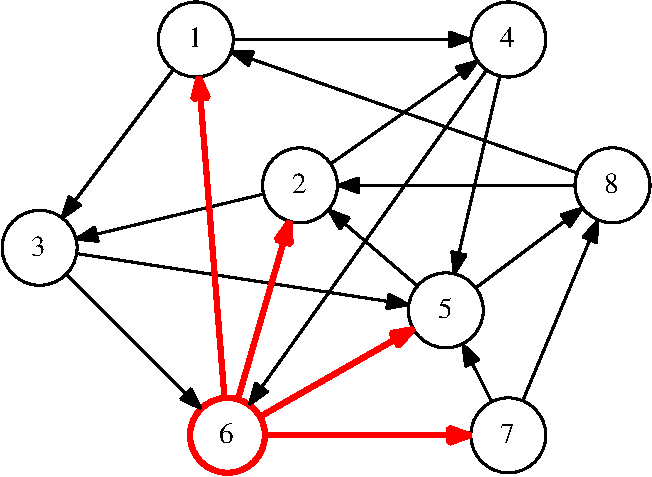
\includegraphics[scale=0.8]{cr-graph-example}
  \caption{An illustration of one step of the process.
  The user is at node 6 and can reach nodes $\mathcal{N}^+_6 = \{1, 2, 5, 7\}$.}
  \label{cr:fig:samplenet}
\end{figure}

To define the transition probabilities, we posit Luce's well-known choice axiom that states that the odds of choosing item $j$ over item $j'$ do not depend on the rest of the alternatives \citep{luce1959individual}.
This axiom leads to a unique probabilistic model of choice.
For every node $i$ and every $j \in \mathcal{N}^+_i$, the probability that $j$ is selected among alternatives $\mathcal{N}^+_i$ can be written as
\begin{align}
\label{cr:eq:singlelik}
p_{ij} = \frac{\gamma_j}{\sum_{k \in \mathcal{N}^+_i} \gamma_k}
\end{align}
for some parameter vector $\bm{\gamma} = [\gamma_1 \ \cdots \ \gamma_N]^\Tr \in \mathbf{R}_{>0}^N$.
Intuitively, the parameter $\gamma_i$ can be interpreted as the strength (or utility) of item $i$.
Note that $p_{ij}$ depends only on the out-neighborhood of node $i$.
As such, the choice process satisfies the Markov property, and we can think of the sequence of choices as a trajectory in a Markov chain.
In the context of this model, we can formulate the inference problem as follows.
Given a directed graph $\mathcal{G} = (\mathcal{V}, \mathcal{E})$ and data on the aggregate traffic at each node, find a parameter vector $\bm{\gamma}$ that fits the data.
